\section{Program}\label{sec:Program}
In this section, I mainly introduce the methods and theories related to programming.  For example, during programming, the library OpenCV is used, but some basic information, like which kind of coordinate it uses for function "warpPerspective", is not included in the documentation of it. So I had to figure them out. What's more,  how to blur images and calculate image derivatives are also mentioned here.  In the end, dyadic program is introduced. 

\subsection{Image Warping}\label{subsec:Image Warping}
In order to do image registration, the function to warp image is needed. In the thesis, I have chosen the library OpenCV for warping images. How to warp the target image to the template image with the calculated homography matrix is a very important step of implementation.

Because homography is a perspective transformation, OpenCV calls the function "warpPerspective" to warp an image with a homography matrix. The function applies a perspective transformation to an image. The introduction of it in OpenCV documentation \cite{opencvdevteamOpenCV13Documentation} is listed here:
\begin{python}[caption={Model of warpPerspective},label={lst:model of warpPerspective}]
	cv2.warpPerspective(src, M, dsize[, dst[, flags[, borderMode[, borderValue]]]])
\end{python}
where
the parameters: 
\begin{itemize}
	\item \textbf{src} - input image
	\item \textbf{M} - $3 \times 3$ homography transformation matrix
	\item \textbf{dsize} - size of the output matrix
	\item \textbf{flags} - combination of interpolation methods(INTER\_LINEAR or INTER\_NEAREST) and the optional flag WARP\_INVERSE\_MAP, that sets $M$ as the inverse transformation ($ dst \rightarrow src $)
	\item \textbf{borderMode} - piexl extrapolation 
	methode (BORDER\_CONSTANT \\ or BORDER\_REPLICATE).
	\item \textbf{borderValue} - value used in case of a constant border; by default, it equals 0.
\end{itemize}
The function transforms the source image using the specified matrix:
\begin{align}
	dst(x, y) = src\left( \frac{M_{11}x + M_{12}y+ M_{13}}{M_{31}x+M_{32}y + M_{33}}, \frac{M_{21}x + M_{22}y + M_{23}}{M_{31}x + M_{31}y + M_{33}} \right)
\end{align}
when the flag "	WARP\_INVERSE\_MAP" in the function is set, Otherwise, the transformation is first inverted with \textbf{invert()} and then put in the formula above instead of \textbf{M}. 

According to this, the target image $I_2$ is put into the function "warpPerspective" as \textbf{src}. And $H_{n} = H_{\infty} + \vec{e} \cdot \vec{q}_{n}^T$ is set as \textbf{M}. And the \textbf{flags} are INTER\_LINEAR and WARP\_INVERSE\_MAP. The output of the function is a warped image which is used to show the estimation result and compare with the template image $I_1$ to get the mapping error $\vec{e}_n$. 

But what we optimize in the program are $H_{\infty}$,  $\vec{e}$ and $ \vec{q}_{n}^T$. There isn't explicit homography matrix $H_n$ in program. In order to warp the image with $H_{\infty}$,  $\vec{e}$ and $ \vec{q}_{n}^T$, a new function based on "warpPerspective" is built to warp the image in the program:
\begin{python}[caption={warp\_image},label={lst:warpimage}]
	def warp_image(q, e, H_inf, target_img, template_img):
		H = H_inf + e @ q.T
		
		width_x = np.array(template_img).shape[1]
		height_y = np.array(template_img).shape[0]
		
		warped_img = cv2.warpPerspective(target_img, H, (width_x, height_y),
		flags=cv2.INTER_LINEAR + cv2.WARP_INVERSE_MAP)
	return warped_img
\end{python}

Although the openCV documentation describes the parameters of functions in detail, the specific description of the coordinate system is not involved. For example, the specific location of the origin, the direction of the coordinate axis, and how to perform homogeneous and dehomogeneous are not clearly indicated. But for image registration technology, accuracy is very important. Therefore, the above problems need to be explored and the program must be adjusted accordingly to ensure accuracy.

First tests with the function reveal that x-axis points right, y-axis points downwards and z-axis for homogenization and dehomogenization of the homogeneous coordinates. But it can be only seen that the origin of pixel coordinate is somewhere on the top left corner. There are two types of pixel coordinate. 
\begin{enumerate}
	\item The origin is at the middle of the upper left corner pixel of the image with the positive Row axis pointing downwards and the positive Column axis pointing towards the right \cite{misbPhotogrammetryMetadataSet}.
	\item The origin is at the upper left corner of the upper left pixel of the image with the positive Line axis pointing downwards and the positive Column axis pointing towards the right \cite{misbPhotogrammetryMetadataSet}.
\end{enumerate}

To clarify this problem, a little test program is used. Assumed that a simple image (shown in \cref{fig:Test Image}) with only 4 pixel, which is 
\begin{align}
\begin{bmatrix}
100&170\\
170&170 
\end{bmatrix} \nonumber
\end{align}
is transformed by a homography matrix
\begin{align}
\begin{bmatrix}
2&0&0\\
0&2&0\\
0&0&1\\
\end{bmatrix} \nonumber
\end{align}
which is corresponds to scale the template image by factor $2$.(In function "warpPerspective", \textbf{flag} WARP\_INVERSE\_MAP is not used in the test.) And if the gray value of a quarter area in the upper left corner in the warped image is $100$, this proves that the origin is at the upper left corner of the upper left pixel of the image in the function "warpPerspective". Otherwise, the type 1 is used. 

The result should is shown in \cref{fig:Result Image}. It's obvious from the result, that the function regards the middle of pixel at upper left corner as the origin of the pixel coordinate. So I will use this definition in the thesis, too.
\begin{figure}[htbp]\centering
	\subfloat[Testing image]{
		\label{fig:Test Image}
		
\includegraphics[width=0.20\textwidth]{images/tofindorigin/img_2_transform.png}
	} \qquad
	\subfloat[Result image]{
		\label{fig:Result Image}
		
\includegraphics[width=0.40\textwidth]{images/tofindorigin/img_form.png}
	} 
	\caption{Origin of the coordinate system used by "warpPerspective"}
	\label{fig:Searching Origin}
\end{figure}

\subsection{Image Pyramid}
In cases, images contain much noise. In image processing, it will influence the result. So before implementation of the algorithm, we must reduce the noise in image. There are some low pass filters, which can be used for image blurring. Here I have chosen the most common filter, Gaussian filter to make a Gaussian blur. In addition, it's also used in the thesis to make a Gaussian pyramid of images to reduce the effects of repeating structure and allow for a large range of convergence of the algorithm.

The proposed algorithm is based on the least square method. Therefore, the less blurry the image, the more noise will be introduced into the iterative process, and the greater the interference to the final result. At the same time, the algorithm will converge slowly because of noise influence. To avoid this problem, image pyramid is used in the program.

Go further, when there is repeating structures (texture) in the target plane such as brick floor, the repetitive structure can be almost blurred away with image pyramid and there is enough other structure left that make the algorithm converge.

In the program, the function "pyrDown" from OpenCV is used to build  Gaussian image pyramid(An example image pyramid built by this function is shown in \cref{fig:iamge pyramid}).
\begin{python}[caption={Image pyramid}, label={lst:Imagepyramid}]
	cv2.pyrDown(src[, dst[, dstsize[, borderType]]])
\end{python}
With this function, an image pyramid as a set of layers in which the higher the layer, the smaller the size is build.

After building an image pyramid of testing image, the algorithm will first calculate at the highest layer of the pyramid, which is the layer with the lowest resolution. When the preliminary result is obtained, it will be re-scaled into next layer and used as the initialization of next layer. With this initialization, the algorithm runs on the next layer. Repeat this until the last layer or the original image. Then the result has no offset and more accurate. At the same time the algorithm converges faster. Because it takes less time to converge, when the algorithm is applied to the lower resolution image. With a prior result for initialization of the higher resolution image, it also reduces the running time of the algorithm.

\begin{figure}[htbp]\centering
	\subfloat[Image in 3rd layer]{
	
		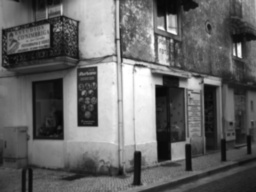
\includegraphics[width = 2cm]{./images/ImagePyramid/template_img_pyramid_of2_layer}
	} \\
	\subfloat[Image in 2nd layer]{

		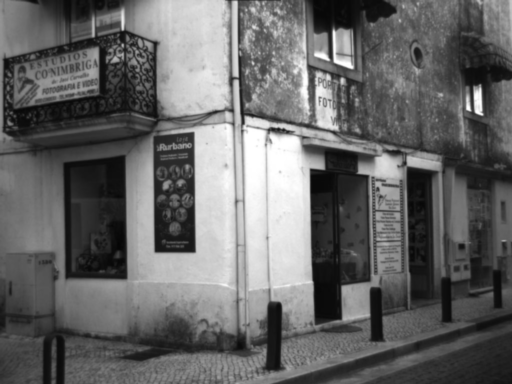
\includegraphics[width = 4cm]{./images/ImagePyramid/template_img_pyramid_of1_layer}
	} \\
	\subfloat[Image in 1st layer]{

	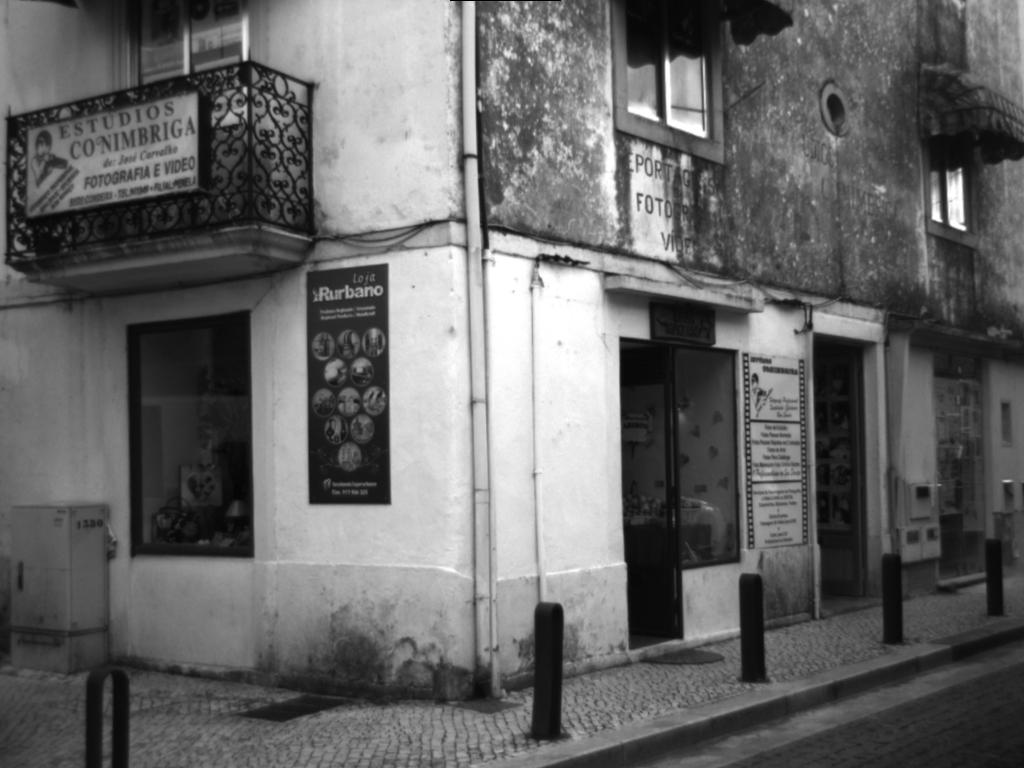
\includegraphics[width = 8cm]{./images/ImagePyramid/template_img_pyramid_of0_layer}
	} 
	\caption{Visual representation of an image pyramid with 3 levels}
	\label{fig:iamge pyramid}
\end{figure}



\subsection{Image Derivatives}\label{sec:Image derivatives}
When talking about the derivative of an image, you're actually talking about what's called a discrete derivative, and it's more of an approximation of the derivative. One simple example is that you can take the derivative in the x-direction at pixel $\rdx'_{ij}$ by taking the difference between the pixel values to the left and right of your pixel. It's widely used in edge detection. But in my thesis, only the first derivation of image is needed to approximate the term $\frac{\mathrm{d} I_2(N)}{\mathrm{d}N}$ in \cref{eq:jnuR}:
\begin{align}
	j_{nu} 
	= \frac{\mathrm{d} I_2(N)}{\mathrm{d}N} \frac{\mathrm{d} N(T_n)}{\mathrm{d} T_n} \frac{\partial T_n(\vec{\beta}, \rdx_{ij})}{\partial \beta_u} \nonumber
\end{align}

In computer version, image derivatives can be computed by using small convolution filters of size $2 \times 2$ or $3 \times 3$, such as Sobel, Roberts and Prewitt operators. However, a large mask will generally give a better approximation of the derivative and examples of such filters are Gaussian derivatives and Gabor filters. Sometimes high frequency noise needs to be removed and this can be incorporated in the filter so that the Gaussian kernel will act as a band pass filter in the process. The most used derivatives filter kernel is shown in \cref{fig:Derivative Filter}.
\begin{figure}[htbp]
	\centering
	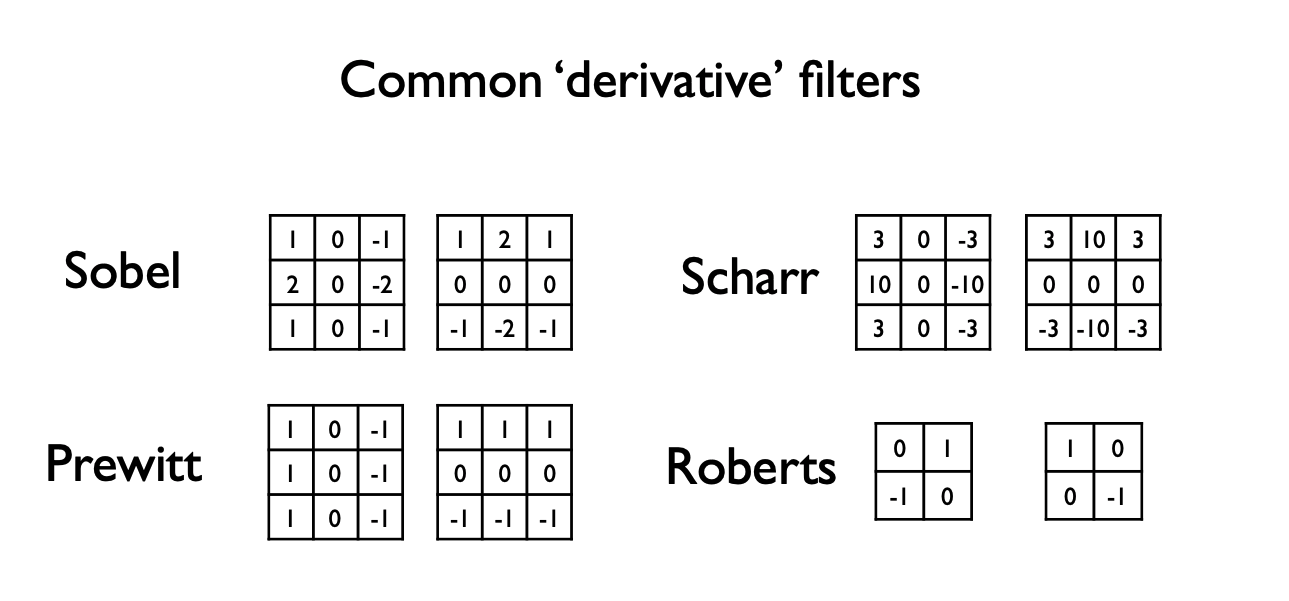
\includegraphics[width=0.80\textwidth]{images/derivatives}
	\caption{Derivative filter}
	\label{fig:Derivative Filter}
\end{figure}

In the Library OpenCV, there is a function "cv2.Sobel" to calculate the first, second, third or mixed derivatives using extended Sobel operator. This is used to calculate the image derivatives in the implementation. 

The Sobel operator uses two $3\times3$ kernel (usually) which are convolved with the original image to calculate approximations of the derivatives - one for horizontal changes, and one for vertical. If we define $A$ as the source image, and $G_x$ and $G_y$ are two images which at each point contain the vertical and horizontal derivative approximations respectively, the computations are as follows \cite{SobelOperator2020}:
\begin{align}
	G_x = \frac{1}{8}\begin{bmatrix} 
		+1 & 0 & -1  \\
		+2 & 0 & -2 \\
		+1 & 0 & -1 
	\end{bmatrix} * A
	\quad
	\mbox{and}
	\quad   
	G_y = \frac{1}{8}\begin{bmatrix} 
		+1 & +2 & +1\\
		0 & 0 & 0 \\
		-1 & -2 & -1
	\end{bmatrix} * A
\end{align}
where $*$ here denotes the 2-dimensional signal processing convolution operation.

The function "cv2.Sobel" in OpenCV \cite{opencvdevteamOpenCV13Documentation}shows:
\begin{python}[caption={Model of Sobel Filter},label={lst:Model of Sobel filter}]
	cv2.Sobel(src, ddepth, dx, dy[, dst[, ksize[, scale[, delta[, borderType]]]]]) 
\end{python}

However, the Sobel operator, while reducing artifacts associated with a pure central differences operator, does not have perfect rotational symmetry.  Scharr looked into optimizing this property. Scharr operators result from an optimization minimizing weighted mean squared angular error in Fourier domain. This optimization is done under the condition that resulting filters are numerically consistent. Therefore, they really are derivative kernels rather than merely keeping symmetry constraints \cite{SobelOperator2020}.

There is also a special value $ksize=CV\_SCHARR(-1)$ of function "cv2.Sobel" that corresponds to the $3\times3$ Scharr filter in function that gives more accurate results than the Soble operator. The Scharr aperture is:
\begin{align}
	\frac{1}{32}\begin{bmatrix}
		-3& 0& 3\\
		-10&0&10\\
		-3&0&3
	\end{bmatrix} \nonumber
\end{align}
for the x-derivative, or transposed for the y-derivative.

The function combine Gaussian smoothing and differentiation, so the result is more or less resistant to the noise. Most often, the function is called with (xorder =1, yorder =0) or (xorder =0, yorder =1) to calculate the first x- or y- image derivative.

In the thesis, what needed in program is $\frac{\mathrm{d} I_2(N)}{\mathrm{d}N} $, with
\begin{align}
		\rdy'_{ij} &= N(\rdy_{ij}) \nonumber \\
		\rdy_{ij} & = (H_{\infty} + \rde \cdot \vec{q}_{n}^T) \rdx_{ij} \nonumber 
\end{align}
The meaning of this term is the derivative of pixel $\rdy'_{ij}$ in image $I_2$. To get this, the exact $\rdy'_{ij}$ corresponding to $\rdx'_{ij}$ should be known. So the function "warp\_image" in \cref{subsec:Image Warping} combining function "cv2.Sobel" can complete this task.  Function "warp\_image" calculates $\rdy'_{ij}$ and function "cv2.Sobel" calculates the derivative. An example is shown below:
\begin{enumerate}
	\item First, use function "cv2.Sobel" function to calculate the first x and y derivative of origin image $I_2$:
\begin{python}[caption={Derivative in x and y direction},label={lst:Model of Sobel Fildaster}]
	ImageDerivativeX = cv2.Sobel(target_img, -1, 1, 0, ksize=-1)
	ImageDerivativeY = cv2.Sobel(target_img, -1, 0, 1, ksize=-1)
\end{python}
\item Then the output of last step should be warped with function "warp\_image" and $H_{\infty}$,  $\vec{e}$ and $ \vec{q}_{n}^T$:
\begin{python}[caption={$\frac{\mathrm{d} I_2(N)}{\mathrm{d}N} $},label={lst:Model of Sdasobel Fildaster}]
	ImageDerivativeX_warp = self.warp_image(q, e, H_inf, ImageDerivativeX, template_img)
	ImageDerivativeY_warp = self.warp_image(q, e, H_inf, ImageDerivativeY, template_img)
\end{python}
\end{enumerate}

\subsection{Dyadic Program}\label{Dyadic Program}
Generally speaking, the images that are the objects of our algorithm contain all millions to ten of millions pixels. So when I apply the algorithm, the dimension of  \cref{eq:J_F} will reach 20 million even more. In this way, when we calculate pseudo-inverse of $\mathbf{J}_{F}$, it will require a very large memory space and running time, which greatly increases the computation time of algorithm. In order to avoid this problem, I will optimize it during programming, so as to improve the reaction speed of the program.

The main idea is to use dyadic product to build a dyadic program. In mathematics, specifically multilinera algebra, a dyadic or dyadic tensor is a second order tensor, written in a notation that fists in with vector algebra. The dyadic product takes in two vectors and returns a second order tensor called a "dyadic". A dyadic can be used to contain physical or geometric information, although in general there is no direct way of geometrically interpreting it.

It also has some aspects of matrix algebra, as the numerical components of vector can be arranged into row and column vectors, and those of second order tensors in square matrix. Dyadic expressions may closely resemble the matrix equivalents.

Here I will use the process of calculating \cref{eq:simple} in step Optimize $\vec{Q}^k, \vec{R}^k$ per patch to explain the details of using dyadic product. In each cycle, the term
\begin{align}
	\left(\mathbf{J}_{F_n+R_n}^{T} \mathbf{J}_{F_n+R_n} \right)^{-1} \mathbf{J}_{F_n+R_n}^{T} \vec{e}_{n} \nonumber
\end{align} 
should be calculated. Rewrite $\mathbf{J_{F_n+R_n}}$ in this form:
\begin{align}
	\mathbf{J_{F_n+R_n}} = \begin{pmatrix}
		B_1^T\\
		B_2^T\\
		\vdots\\
		B_{i\times j}^T
		\end{pmatrix}
\end{align}
where 
\begin{align}
	B_{i \times j}^T &= \begin{pmatrix}\frac{\mathrm{d} I_2(N)}{\mathrm{d}N}\cdot \frac{\mathrm{d} N(T_n)}{\mathrm{d} T_n}\cdot \frac{\partial T_n(\vec{q}_n, \rdx_{ij})}{\partial \vec{q}_n}&- \frac{\partial R_n(I_1(N(\rdx_{ij})))}{\partial {r_1}_n} & - \frac{\partial R_n(I_1(N(\rdx_{ij})))}{\partial {r_2}_n} \end{pmatrix}\\
	&= \begin{pmatrix} b_{i \times j}^{(1)} & b_{i \times j}^{(2)} & b_{i \times j}^{(3)}\end{pmatrix}
\end{align}
with 
\begin{align}
b_{i \times j}^{(1)} &= \frac{\mathrm{d} I_2(N)}{\mathrm{d}N}\cdot \frac{\mathrm{d} N(T_n)}{\mathrm{d} T_n}\cdot \frac{\partial T_n(\vec{q}_n, \rdx_{ij})}{\partial \vec{q}_n} \nonumber \\
b_{i \times j}^{(2)} & = - \frac{\partial R_n(I_1(N(\rdx_{ij})))}{\partial {r_1}_n} \nonumber \\
b_{i \times j}^{(3)}&= - \frac{\partial R_n(I_1(N(\rdx_{ij})))}{\partial {r_2}_n} \nonumber 
\end{align}
and $b_{i \times j}^{(1)}$ is a $1 \times 3$ vector, $b_{i \times j}^{(2)}$ and $b_{i \times j}^{(3)}$ are both scalar each. So the dimension of $B_{i \times j}^T $ is $1 \times 5 $ in this case

So the term $\mathbf{J}_{F_n+R_n}^{T} \mathbf{J}_{F_n+R_n} $ looks like 
\begin{align}
	\mathbf{J}_{F_n+R_n}^{T} \mathbf{J}_{F_n+R_n} &= \begin{pmatrix} B_1 & B_2 & B_3& \cdots & B_{i \times j} \end{pmatrix} \cdot \begin{pmatrix}
		B_1^T\\
		B_2^T\\
		\vdots\\
		B_{i\times j}^T
	\end{pmatrix}
	& = \sum_{1}^{i \times j} B_{s} \cdot B_{s}^T
\end{align}
And $M$ is defined as a temporary represent of $\mathbf{J}_{F_n+R_n}^{T} \mathbf{J}_{F_n+R_n}$  and is initialized as zero matrix $M_0$ with the same dimension of term $B_{s} \cdot B_{s}^T$ (For Optimize $\vec{Q}^k, \vec{R}^k$, it's $5 \times 5$). So for each pixel in the plane patch $n$, $M_s$ can be calculated by accumulating:
\begin{align}
 M_s = M_{s-1} + B_{s} \cdot B_{s}^T
\end{align}
After addition of all pixels in the plane patch $n$, $M_{i \times j} = \mathbf{J}_{F_n+R_n}^{T} \mathbf{J}_{F_n+R_n}$. In this way, the matrix multiplication is changed to addition with dyadic product $ \sum_{1}^{i \times j} B_{s} \cdot B_{s}^T $.

At the same time apply this method to term $\mathbf{J}_{F_n+R_n}^{T} \vec{e}_{n}$, and get the result $W_{i\times j}$ (Here it's a $5 \times 1$ vector.) with the same form of $M_{i \times j}$. Then the final result can be got:
\begin{align}
		\left(\mathbf{J}_{F_n+R_n}^{T} \mathbf{J}_{F_n+R_n} \right)^{-1} \mathbf{J}_{F_n+R_n}^{T} \vec{e}_{n} = M_{i \times j}^{-1} \cdot W_{i\times j}
\end{align}
for plane patch $n$. In each iteration step, only a storage space of matrix with the same dimension of $B_{s} \cdot B_{s}^T$ replace a storage space of matrix with $i \times j$ times dimensions. With this optimization, the speed of matrix inversion is also greatly reduced. One example of code implementation for rectified case is shown below: ( This function only show a single loop in iterative calculation of Optimize $\vec{Q}^k, \vec{R}^k$.)
\begin{python}[caption={Dyadic product example},label={lst:Dyadic Product Example}]
def improve_parameter(self, q, e, H_inf, r_correct, target_img, template_img, *correspondings_field):
	
	M = zeros((5, 5))
	W = zeros((5, 1))
	
	# warp_image is a function which I use warpPerspective to build, to warp the image.
	warped_img = warp_image(q, e, H_inf, target_img, template_img)
	
	ImageDerivativeX = Sobel(target_img, -1, 1, 0, ksize=-1)
	ImageDerivativeX_warp = warp_image(q, e, H_inf, ImageDerivativeX, template_img)
	ImageDerivativeY = Sobel(target_img, -1, 0, 1, ksize=-1)
	ImageDerivativeY_warp = warp_image(q, e, H_inf, ImageDerivativeY, template_img)
	
	for field in correspondings_field:
		x_min_improve = field[0]
		x_max_improve = field[0] + field[1]
		y_min_improve = field[2]
		y_max_improve = field[2] + field[3]
		for y in range(y_min_improve, y_max_improve, 1):
			for x in range(x_min_improve, x_max_improve, 1):
				# coordinate in template img
				x_ij = np.array([[x],[y],[1]])
				
				# dimension fo H is 3*3
				H = (H_inf + e @ q.T) @ x_ij
				
				# dimension of D_N is 2*3
				D_N = np.array([[1, 0, 0], [0, 1, 0]]) / H[2] - np.matmul(H[0:2], np.array([[0, 0, 1]])) / (H[2] * H[2])
				
				# Derivative of I_2 (warped img)
				D_I_12 = np.array([ImageDerivativeX_warp[y, x], ImageDerivativeY_warp[y, x]]).reshape(1, 2)
				
				# D_I after dehomogenous 1*3
				D_I_dehomogenous = D_I_12 @ D_N
				
				# B_1 is the part for Delta p in A_matrix. Dimension is 1 * 3
				B_1 = D_I_dehomogenous @ e @ x_ij.T
				
				# B_2 is the part for Delta a and Delta b in A_matrix. Dimension is 1 * 2
				B_2 = np.array([[template_img[y, x], 1]])
				
				# B is the factor of variable, dimension is 1*5
				B = np.concatenate((B_1, -B_2), axis=1)
				
				# difference between template image and warped image
				d = r_correct[0, 0] * int(template_img[y, x]) + r_correct[1, 0] - int(warped_img[y, x])
				
				# dimension of M_matrix is 5 * 5
				# dimension of W_matrix is 5 * 1
				M = M + B.T @ B
				W = W + d * B.T
	
	# dimension of q is 5 * 1. pinv is pesudo-inverse
	Delta = np.linalg.pinv(M) @ W
	
	return Delta
\end{python}









